\documentclass[11pt, twoside, reqno]{article}
\usepackage{amssymb, amsthm, amsmath, amsfonts}
\usepackage{graphicx}
\usepackage{amsrefs}
\usepackage{color}
\usepackage{hyperref}
\usepackage{bardtex}

\styleoption{juniorseminar}

%your macros, if you have any


\begin{document}

\titlepgjrsem{Mathematics is Fun}{Angela Albee}
    {May}{2099}

\abstr

The abstract should be brief, and non-technical.  Try to minimize the use of symbols in the abstract, so that you can use the abstract elsewhere.

\tableofcontents

\startmain

\section{A Terrific Section}
\label{secA1}

In the Junior Seminar style, there are no chapters, only sections.

\thm\label{thmAA} 
Let $\func fAB$ be a function.
%
\enum 
\item\label{thmAA1}
If $f$ has an inverse, then the inverse is unique.
%
\item\label{thmAA2}
If $f$ has a right inverse $g$ and a left inverse $h$, then $g = h$; hence $f$ has an inverse.
%
\item\label{thmAA3}
If $f$ has an inverse $g$, then $g$ has an inverse, which is $f$.
\eenum
\ethm
 
\demo
(\ref{thmAA1}). Suppose that $\func {g, h}BA$ are both inverses of $f$.  We will show that $g = h$.  By hypothesis on $g$ and $h$ we know, among other things, that $f \circ g = 1_B$ and $h \circ f = 1_A$.  Using a previous lemma we see that
%
\[
g  =  1_A \circ g  =  (h \circ f) \circ g  =  h \circ (f \circ g)  =  h \circ 1_B  =  h.
\]

\noindent (\ref{thmAA2}). The proof is virtually the same as in Part~(1).  
\smallskip

\noindent (\ref{thmAA3}).  Since $\func gBA$ is an inverse of $f$, then $g \circ f = 1_A$ and $f \circ g = 1_B$.  By the definition of inverses, it follows that $f$ is an inverse of $g$.  By Part~(1) of this theorem, we know that $f$ is the unique inverse of $g$.
\edemo


\section{A So So Section}
\label{secAB}

Whenever possible, break the material up into smaller sections.

Also whenever possible, insert figures to aid the reader.  Always refer to the figures in the text.  We see the logo of the Mathematics Program at Bard in Figure~\ref{figMATHBARD}.

\begin{figure}[ht]
\centering
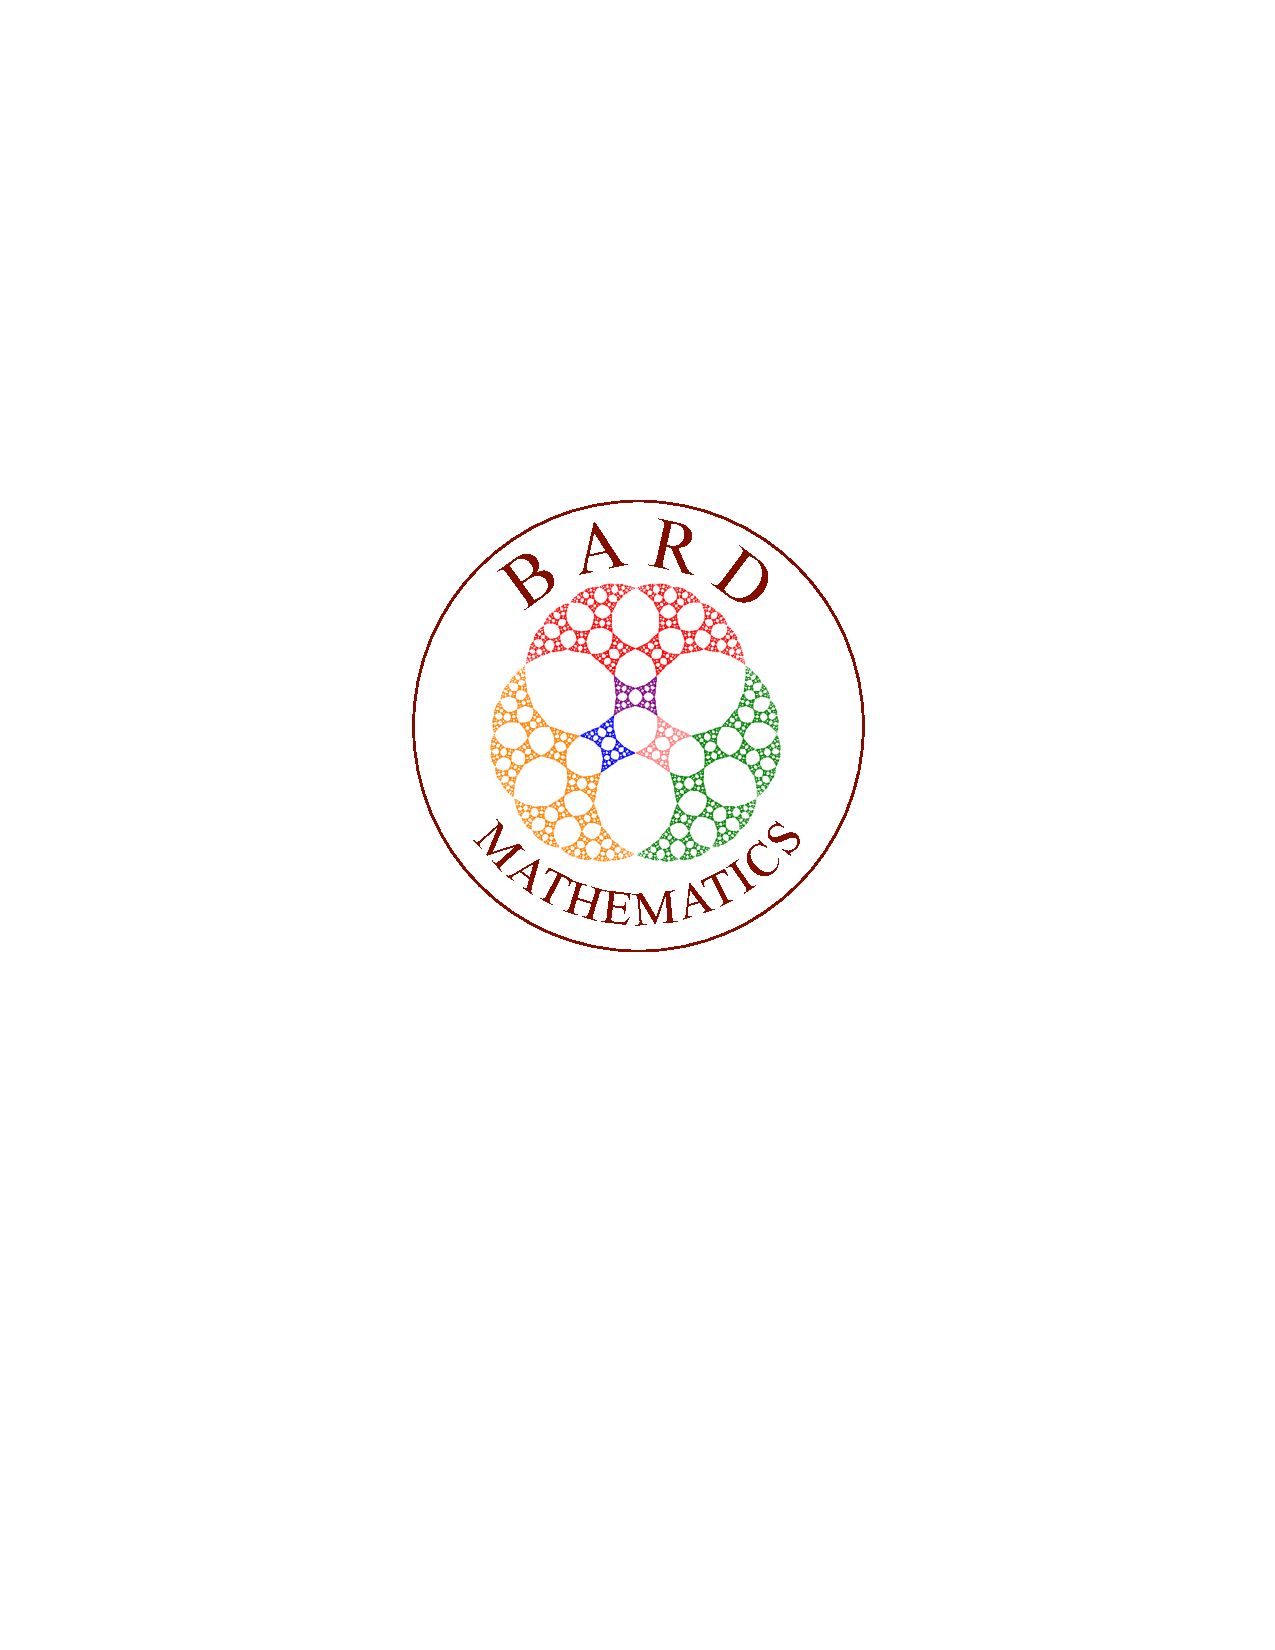
\includegraphics[scale=0.75]{math_prog_logo.pdf}
\caption{The Bard Mathematics Program Logo}
\label{figMATHBARD}
\end{figure}


\subsection{Subsections are Nice}
\label{subsecAB1}

Subsections are available when needed.


\begin{bibliog}

\bib{HOMOLOGY}{book}{
author = {Homology, Harold},
title = {Algebraic Topology for Dummies},
publisher = {Math Lights},
address = {Simplicialville, NY},
date = {2099}
}

\bib{CALCULUS}{article}{
author = {Calculus, Cathy},
title = {Why everyone should love calculus},
journal = {Journal of Fun Mathematics},
volume = {314},
date = {2099},
pages = {100--101}
}

\bib{[PROJECT]}{report}{
author = {Function, Felicity},
author = {Tangent, Tim},
title = {How to Write a Great Junior Seminar Project in Mathematics},
eprint = {http://www.www.www.edu}
}

\end{bibliog}

\end{document}

% end of file bardjuniorsem_template.tex
